\documentclass{report}


\usepackage{style/arxiv}

\usepackage[utf8]{inputenc} % allow utf-8 input
\usepackage[T1]{fontenc}    % use 8-bit T1 fonts
\usepackage{hyperref}       % hyperlinks
\usepackage{url}            % simple URL typesetting
\usepackage{booktabs}       % professional-quality tables
\usepackage{amsfonts}       % blackboard math symbols
\usepackage{nicefrac}       % compact symbols for 1/2, etc.
\usepackage{microtype}      % microtypography
\usepackage{lipsum}
\usepackage{amssymb, amsmath}
\DeclareMathOperator*{\argmax}{argmax} % thin space, limits underneath in displays


% to insert images:
\usepackage{graphicx}
\usepackage{caption}
\usepackage{subcaption}
\usepackage{float} % Necessario per inserire immagini flottanti
% \usepackage{subfigure} % Consente l'inserimento di sottofigure

\DeclareCaptionType{equ}[][]


\newenvironment*{emptyenv}{}{}



\title{Data Intelligence Applications \\
Pricing \& Advertising}


\author{
Andrea Bionda \\
Department of Computer Science and Engineering\\
Politecnico di Milano\\
\texttt{andrea.bionda@mail.polimi.it} \\
\And
Damiano Derin \\
Department of Computer Science and Engineering\\
Politecnico di Milano\\
\texttt{damiano.derin@mail.polimi.it} \\
\And
Andrea Diecidue \\
Department of Computer Science and Engineering\\
Politecnico di Milano\\
\texttt{andrea.diecidue@mail.polimi.it} \\
\And
Antonio Urbano \\
Department of Computer Science and Engineering\\
Politecnico di Milano\\
\texttt{antonio.urbano@mail.polimi.it} \\
\And
Enrico Voltan \\
Department of Computer Science and Engineering\\
Politecnico di Milano\\
\texttt{enrico.voltan@mail.polimi.it} \\
%% \AND
%% Coauthor \\
%% Affiliation \\
%% Address \\
%% \texttt{email} \\
%% \And
%% Coauthor \\
%% Affiliation \\
%% Address \\
%% \texttt{email} \\
%% \And
%% Coauthor \\
%% Affiliation \\
%% Address \\
%% \texttt{email} \\
}

\begin{document}
    \maketitle


    \begin{abstract}
    The goal of the project is to model a scenario in which a seller exploits advertising tools in order to attract more and more users to its website, thus increasing the number of possible buyers.

    The seller has to learn simultaneously the conversion rate and the number of users the advertising tools can attract.

    In this report, we walk through the description of the specific scenario we have studied and the definition of the algorithm design choices we adopted in order to reach our goal.
    Then the achieved experimental results will be presented via some useful plots and
    a final conclusion summarizing the whole work.
\end{abstract}
% keywords can be removed
% \keywords{First keyword \and Second keyword \and More}

    \newpage

    \tableofcontents
    \newpage

    \chapter{Introduction: Scenario Setup}
We have studied a possible real world scenario in which a seller wants to increase the number of possible buyers by exploiting advertising tools.

The product we have considered is a particular pair of shoes which has a production cost (without loss of generality we can assume that the production cost is null) and a sell price.

The analyzed campaign consists of three sub-campaigns, each with a different ad to advertise the product and each targeting a different class of users. Each class is defined by the values of pre-defined features.

The feature space we have considered is characterized by two binary features: 
\begin{itemize}
\item \textit{Age<30} or \textit{Age>30}
\item \textit{Profession} that can be either \textit{student} or \textit{worker}
\end{itemize}

So according to the values of the above described features, we can distinguish among the following classes of users:
\begin{itemize}
\item \textit{Elegant}: a worker with age>30
\item \textit{Casual}: a student with age<30
\item \textit{Sport}: a worker with age<30
\end{itemize}

In each section we have executed 25 experiments and taken the average of all results to evaluate the performances of our algorithms.
Further analyses of these evaluations will be explained in the relative sections.
 % Introduction
    \newpage
    \chapter{Advertising: Clicks Maximization}

In this section we focus on the advertising and more precisely on the clicks maximization problem.\\
The goal of this part is to optimize the budget allocation over the three sub-campaigns in order to maximize the total number of clicks we can get.\\
In particular given the assignment~\ref{assPart2} we have designed a combinatorial bandit algorithm for addreassing this task.\\
In the following chapter we are going to:
\begin{itemize}
	\item describe the environment setup;
	\item explain the algorithm design choice;
	\item comment the obtained results.
\end{itemize}

\section{Environment}
The \textbf{Environment} returns the reward associated to each sub-campaign, by iterating over the days for the entire time horizon.\\
In our setting, it computes the optimal number of clicks knowing the real functions, one for each sub-campaign, generating  the number of clicks given a bid value \textbf{\textit{n(x)}}:\\

\begin{equation}
	n(x) = c_{M} \cdot (v_{M} - e^{-\alpha x})
\end{equation}

where:
\begin{itemize}
	\item $c_{M}$ : is the maximum number of clicks the considered sub-campaign can reach in a day;
	\item $v_{M}$ and $\alpha$ : are values associated to each sub-campaign defining the actual bidding curve.
\end{itemize}


The Environment, given the index of the bid chosen by the Learner, returns the collection of rewards associated to each sub-campaign in a completely transparant way to the learning algorithm.\\
How the learner works and its implementation will be described in the following section.



\section{Algorithm Design Choices}

This section deals with the description of the algorithm design choices we adopted and
it also contains the most relevant reference to the code.\\
In the class \textit{BiddingEnvironment.py}, which extends the class \textit{Environment.py} we have defined the actual environment we are working in, described in section before, with the definition of the bids space and the three curves \textit{n(x)}.\\
In order to find the best budget allocation over the three sub-campaigns able to maximize the total number of clicks, we have designed a combinatorial bandit algorithm.\\
In the first phase of the algorithm, we learn the model of each sub-campaign from the observation we get.
To do that in \textit{GP\_Learner.py} we have used a \textit{Gaussian process regressor}.\\
Afterward, the model of each sub-campaign is updated using those observations and the GP will reduce the uncertainty of its estimation. In this way, for each new collected sample, the function estimated by the GP approaches to the real function.\\


In order to properly used a GP regressor, we had to normalize the data. The bid space was already defined in range [0,1] and so the input variable has not to be normalized. So, we only needed to normalize the target and we have done it in the construction of the gaussian process.\\
A Gaussian proccess is completely defined by its mean and its covariance.Since we don't have any prior information we assumed to have zero mean and the covariance given by the squared exponential kernel function \textbf{k(x,x')}:
\begin{equation}
	k(x,x') = \theta^{2} e^{-\frac{(x-x')^2}{2 l^2}}
\end{equation}
where:
\begin{itemize}
	\item \textit{l} :is the \textit{lengthscale};
	\item $\theta$: is the \textit{scale factor}
\end{itemize}
The optimal value of the two hyperparameters have been found by maximiziation of the marginal likelihood during the fit proccess.
\\
\\
In the second phase of the algorithm we have used the values from the learned model to solve the problem of finding the best budget allocation to be set for the current day.\\
In the \textit{Optimizer.py} class we have implemented a modified version of the dynamic programming algorithm used for solving the knapsack problem.\\
More precisely,we have used a matrix in which each row represents the fact that at each step a new sub-campaign enters the problem, while for the columns we have discretized the whole budget in 20 possible uniformly distributed combinations of the budget allocation.\\
Each cell of the matrix contains the value of the best allocation for the considered row and column. 
The result is given by the maximization of the sum of the values provided by the best solution of the problem solved in the previous row (i.e. without considering the new entered sub-campaign) and 
the value of the new considered sub-campaign (considered singularly) s.t. the daily budget over the three sub-campaigns sums to the total daily budget.\\
Once we have filled the entire table, we have the best solution in the last row, i.e. when all the 3 sub-campaigns are considered.\\
In figure ~\ref{curve2Fig} we can see, for each sub-campaign, the real function generating the number of clicks n(x), the function learned by GP regressor and its associated uncertainty.

\begin{figure}[!htb]
	\centering
	%\captionsetup{justification=centering,margin=1cm}
	
	\begin{subfigure}[!H]{0.8\textwidth}
		\centering
		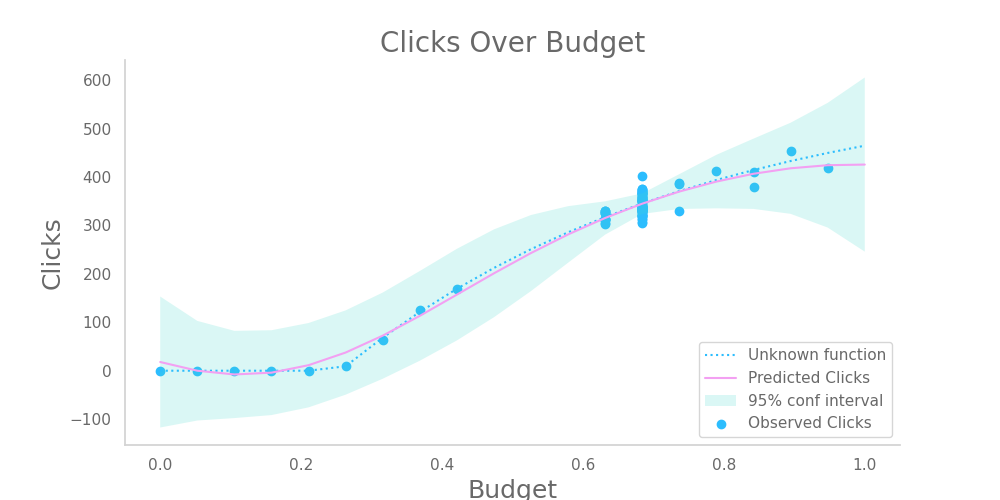
\includegraphics[width=\textwidth]{images/part2_bidding_curve_subcamaign_0.png}
	\end{subfigure}
	
	\begin{subfigure}[!H]{0.8\textwidth}
		\centering
		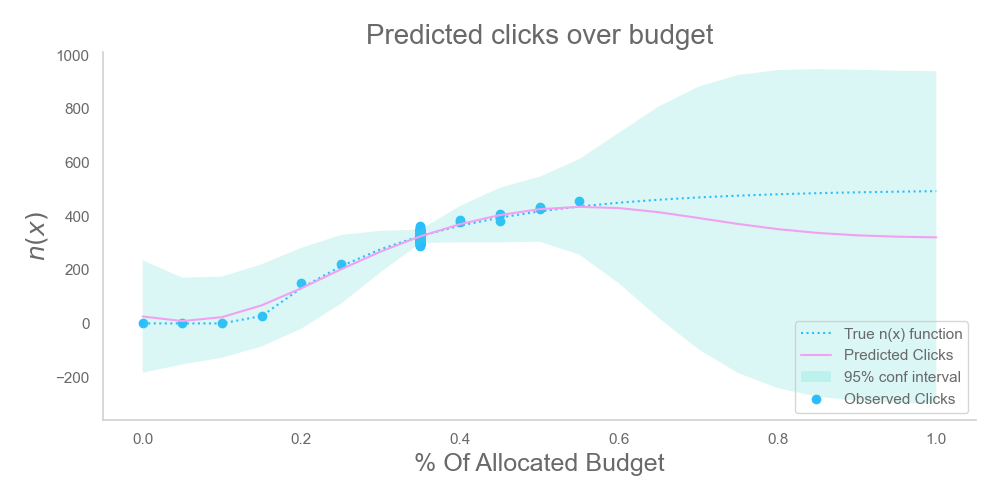
\includegraphics[width=\textwidth]{images/part2_bidding_curve_subcamaign_1.png}
	\end{subfigure}
	%\hfill
	\begin{subfigure}[!H]{0.8\textwidth}
		\centering
		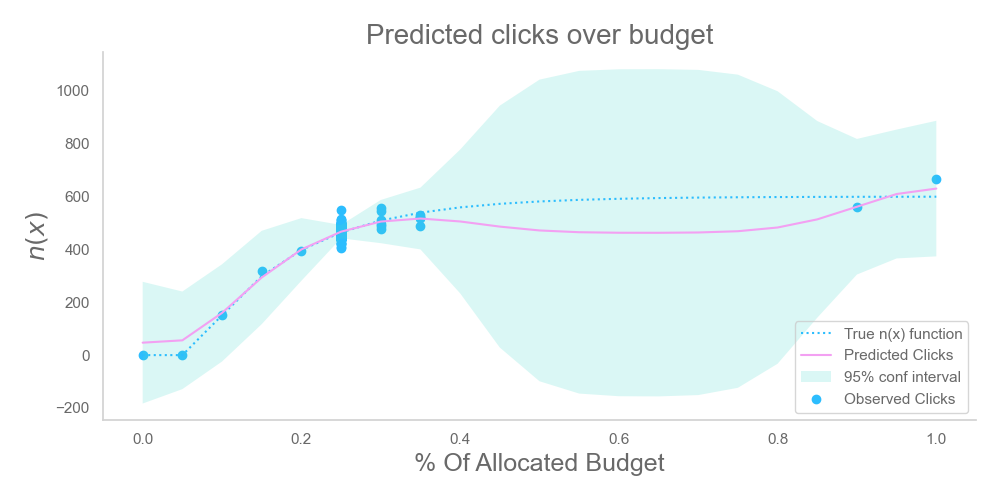
\includegraphics[width=\textwidth]{images/part2_bidding_curve_subcamaign_2.png}
	\end{subfigure}

	\caption{Functions generating the number of clicks}.
	\label{curve2Fig}
\end{figure}

\section{Performance evaluation}
In order to evaluate the performance of the implemented algorithm, we have computed the \emph{cumulative regret} as the difference between the expected reward of the \textit{Clairvoyant algorithm} and the expected reward of our combinatorial bandit algorithm.\\
In \ref{regret2Fig} the plot of the regret we obtain:
\begin{figure}[!htb]
	\centering
	%\captionsetup{justification=centering,margin=1cm}
		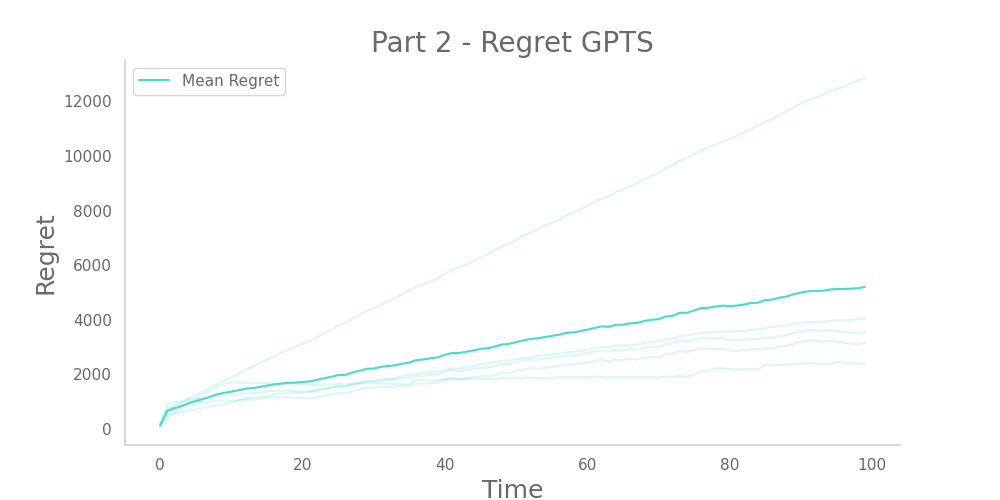
\includegraphics[width=\textwidth]{images/part2.png}
	\caption{Cumulative regret of the combinatorial bandit algorithm}.
	\label{regret2Fig}
\end{figure}



    \newpage
    \chapter{Advertising: Handling Abrupt Phases}

The object of this section is to optimize the budget allocation over the three sub-campaigns in order to maximize the total number of clicks in the case in which there are the three abrupt phases.
For addressing this assignment [\ref{assPart3}] we started from the simplified case of one single phase solved in the previous section and we extended it, by implementing a sliding-window combinatorial bandit algorithm, in order to take in consideration the more general scenario of multiple phases.\\


\section{What is an abrupt phase}
Abrupt changes are a specific case of non stationary environment.
In non stationary environments the probability distribution of the random variable associated with the reward of every arm can change during time.
Abrupt changes are typically associated to new products enter in the market. In this scenario the interests of the customers toward the previous goods can decrease drastically.
In this particular environment the total time horizon is divided in phases and in every phase the reward function is constant while it changes abruptly between the end of a phase and the beginning of the next one.\\ In Figure \ref{abruptFigure} we can see an example of three different curves generating the number of clicks, one for each phase, associated to a specific sub-campaign.
\begin{figure}[!htb]
    \centering

    \minipage{0.48\textwidth}
    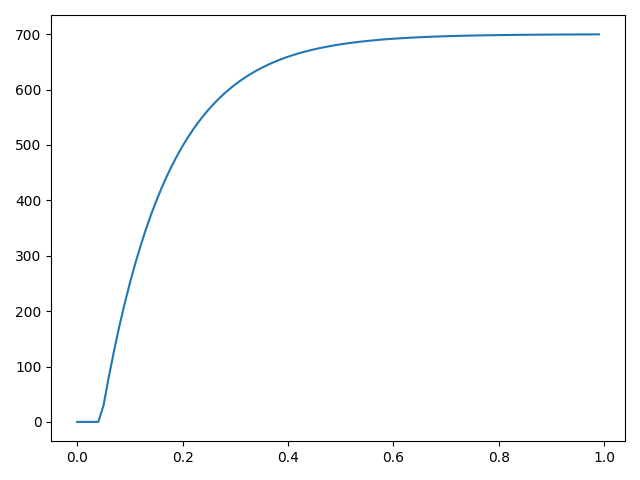
\includegraphics[width=\linewidth]{images/phase0.png}
    \endminipage\hfill
    \minipage{0.48\textwidth}
    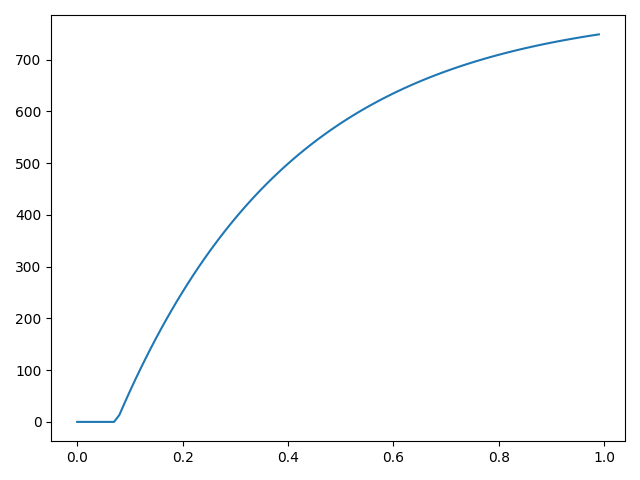
\includegraphics[width=\linewidth]{images/phase1.png}
    \endminipage\hfill
    \minipage{0.48\textwidth}
    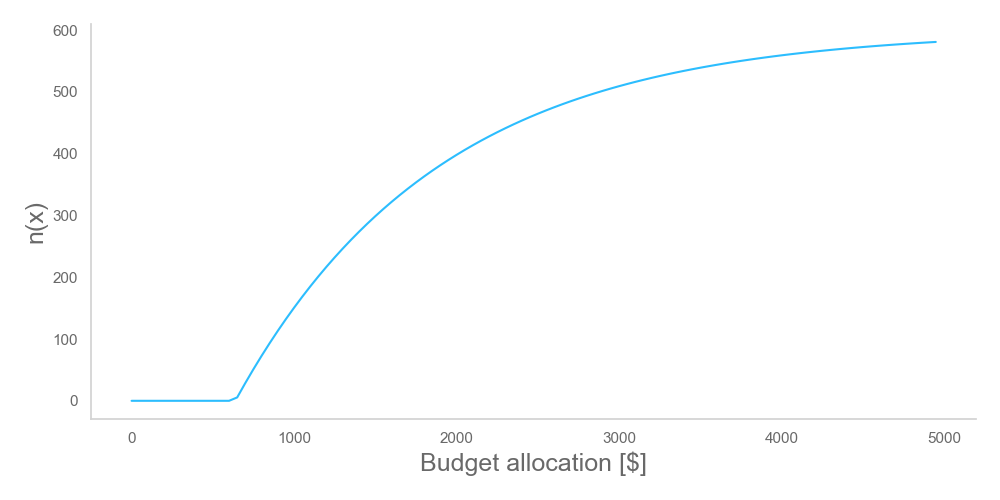
\includegraphics[width=\linewidth]{images/phase2.png}
    \endminipage\hfill

    \caption{Example of different curves associated to different abrupt changes}
    \label{abruptFigure}
\end{figure}


\section{Sliding window mechanism}
For this purpose we have implemented the \textit{Abrupt Bidding Environment} class which extends the \textit{Bidding Environment} class. This class works in a scenario of multiple abrupt phases by returning, for each sub-campaign, the reward of a given pulled arm, depending on the phase we are in.

In this case, the functions generating the number of clicks given a bid value can change dynamically, according the phase we are in.
The curves differ from the previous definitions only for the dependence to the phase we are in. As follows the mathematical definition of the three curve functions:

\begin{equation}
    n(x) = c_{M}[phase] \cdot (v_{M}[phase] - e^{-\alpha x})
\end{equation}

We have to remark that the learner is completely transparent with respect to the phase we are in and in order to learn the three curves in the case of multiple abrupt phases, we have implemented the \textit{Dynamic Learner (DL)} class as an extension of the standard GP Learner.
It implements a \textit{sliding window} mechanism in which we pull a new arm and add the collected rewards until the length of the window is reached. When the window is full, for each new pulled arm we get, we delete the last recent value and add the new one to the collected rewards.\\ Before comparing the performance of this implementation with respect to the one of the standard GP Learner, we did a validation in order to understand what is the best length of the window to be adopted. In Figure \ref{winLenValidationFig} the regret associated to three different example of executions of the algorithm with a different windows length. In particular in the plots we can see the regrets in which the length has been set to 33, 67 and 133, i.e. respectively $\frac{1}{6}$, $\frac{1}{3}$ and $\frac{2}{3}$ of the whole time horizon T = 200 days.
\begin{figure}[!htb]
    \centering

    \minipage{0.48\textwidth}
    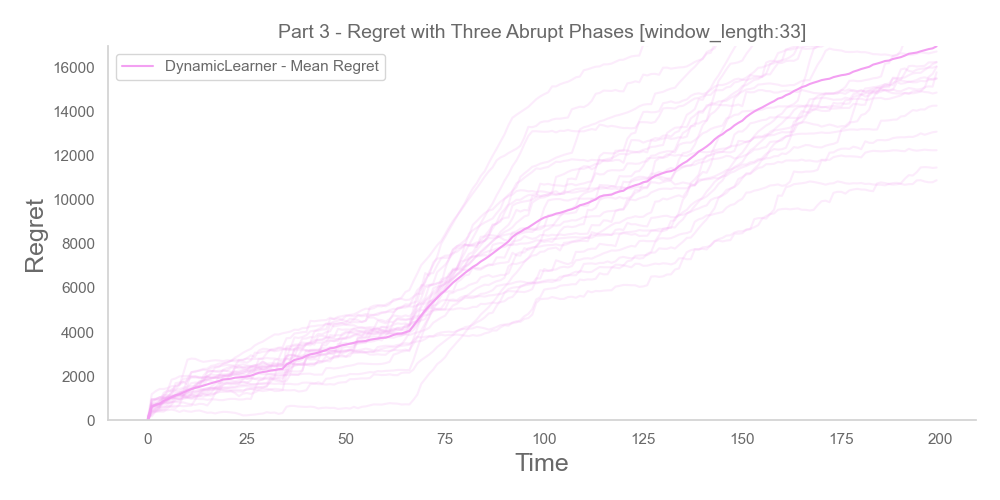
\includegraphics[width=\linewidth]{images/win_length33.png}
    \caption{Window length = 33}\label{win33}
    \endminipage\hfill
    \minipage{0.48\textwidth}
    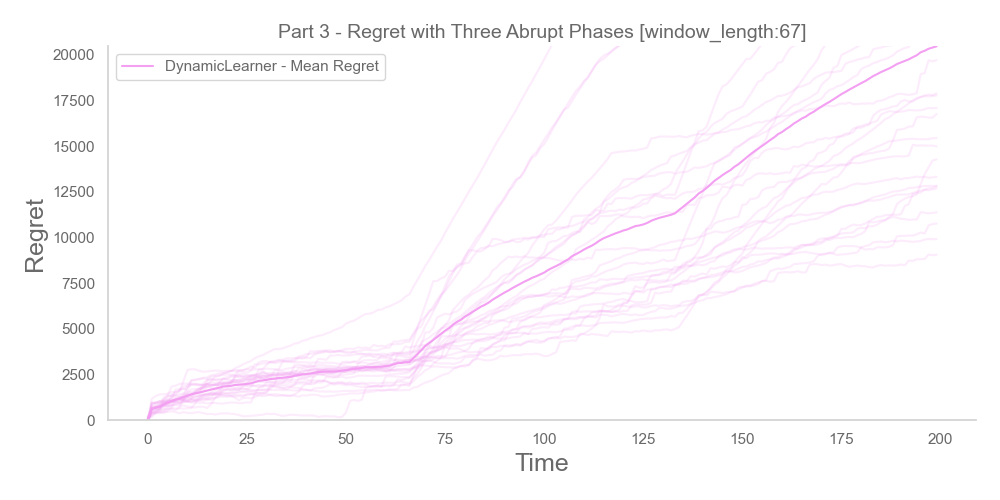
\includegraphics[width=\linewidth]{images/win_length67.png}
    \caption{Window length = 67}\label{win67}
    \endminipage\hfill
    \minipage{0.48\textwidth}
    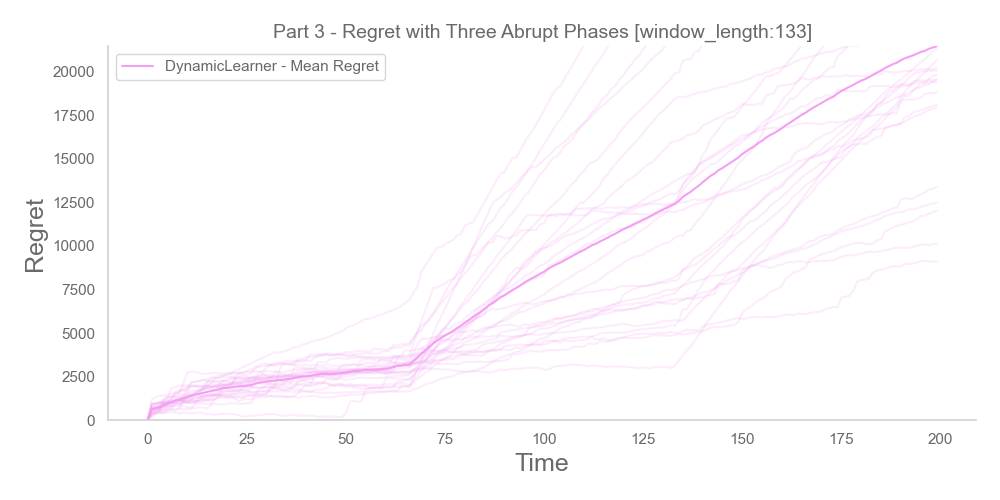
\includegraphics[width=\linewidth]{images/win_length133.png}
    \caption{Window length = 133}\label{win133}
    \endminipage\hfill

    \caption{Tuning in order to find the best window length value.}
    \label{winLenValidationFig}
\end{figure}


As we can notice the performance is highly influenced by the choice of the window length value.
Furthermore all the above results are obtained by running the algorithm over three phases characterized by the same length and so the result can differing more in less specific scenario. For this reason a new method has been designed and implemented to overcome this problem.\\
The final results of the performance of the sliding windows algorithm is for this postponed and it will be analyzed in the last section, after the description of the new algorithm we propose.


\section{Changes Detection mechanism}

For solving this problem we have implemented an innovative method which is based on the concept of the \textit{Statistical test}.
We recall that a statistical test is a procedure for deciding whether a hypothesis about a quantitative feature of a population is true or false. Then for testing a hypothesis, we draw a random sample and calculate an appropriate statistic on its items. If, in doing so, we obtain a value of the statistic that would occur rarely when the hypothesis is true, we would have reason to reject the hypothesis.

In our scenario, to detect changes, we need to compare the value of the new drawn sample with the distribution of the points belonging to the same arm in order to decide whether the hypothesis $H_0$,that the new drawn point belongs to that distribution, is true.
Let us suppose to draw a sample whose value is $x_0$ and let $\mu$ and $\sigma^2$ be respectively the average
and the standard deviation of the the distribution of the points belonging to the pulled arm.
If the point doesn't belong to that distribution the hypothesis test should reject $H_0$, with a \textit{confidence interval of 99\%} So we have:

\begin{equation}
    \mathbb{P}\left(\frac{|x_0 - \mu|}{\sqrt{\sigma^2}} > h \right) = 0.01
\end{equation}

We have that the critical z-score when using a 99\% confidence level are $\pm 2.58$ standard deviations.\\

In the \textit{DL Change Detect} class, we have implemented such change detector. When an arm is pulled more than '\textbf{min\_len}' \footnote{min\_len indicates the minimum number of data we need to have in an arm in order to consider reasonable to run the test} times, for each pull we run the statistical test. When the test reject $H_0$, it means that the point doesn't belong to that distribution and so it means that it is changed. In this case we reset the arm.\\
As we did for the sliding window case, also for this algorithm we performed some validation, in order to understand how to properly set the value of the \textit{min\_len}. As follows the plots of the regrets associated to three different example of executions of the algorithm by changing the value of the hyperparameter, i.e. with min\_len equal to 3, 6 and 10 respectively in Fig \ref{minlen3}, \ref{minlen6}, \ref{minlen10}

\begin{figure}[!htb]
    \centering

    \minipage{0.48\textwidth}
    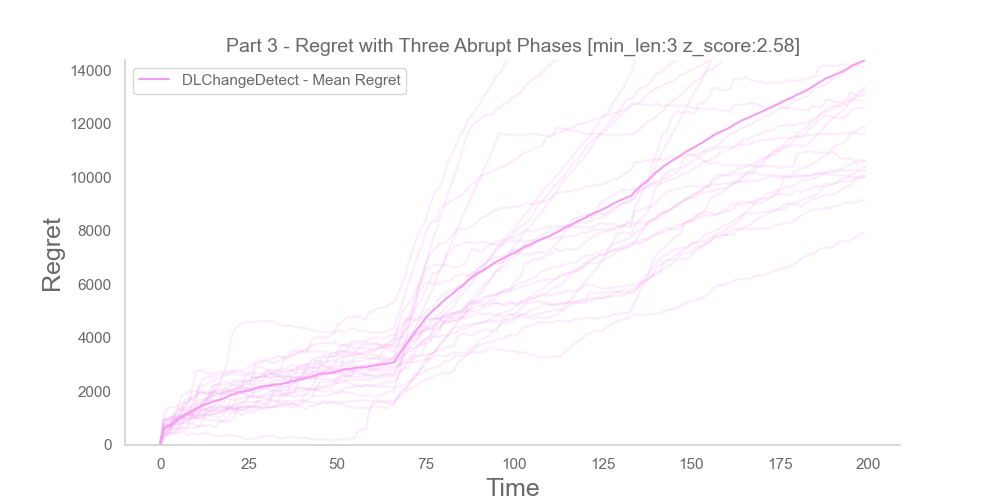
\includegraphics[width=\linewidth]{images/part3_min-len3_z_score2_58.png}
    \caption{case of min\_len = 3}\label{minlen3}
    \endminipage\hfill
    \minipage{0.48\textwidth}
    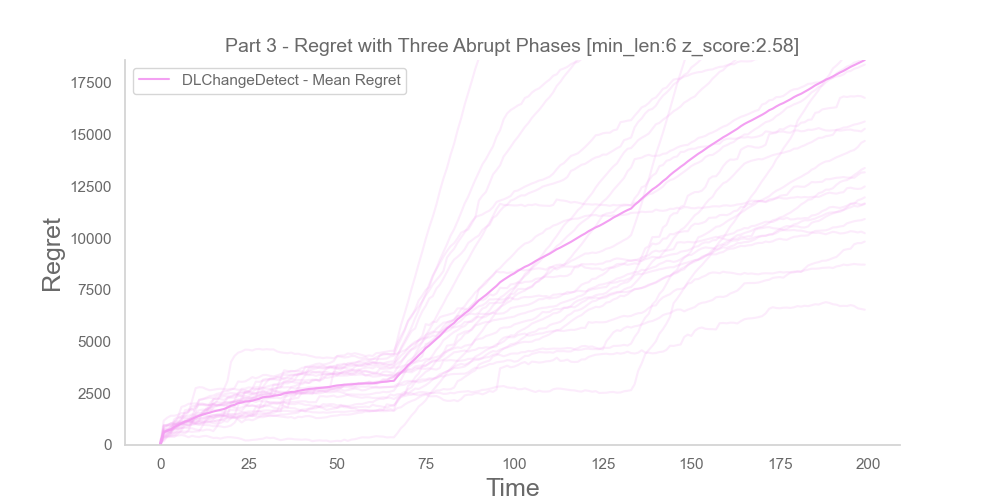
\includegraphics[width=\linewidth]{images/part3_min-len6_z_score2_58.png}
    \caption{case of min\_len = 6}\label{minlen6}
    \endminipage\hfill
    \minipage{0.48\textwidth}
    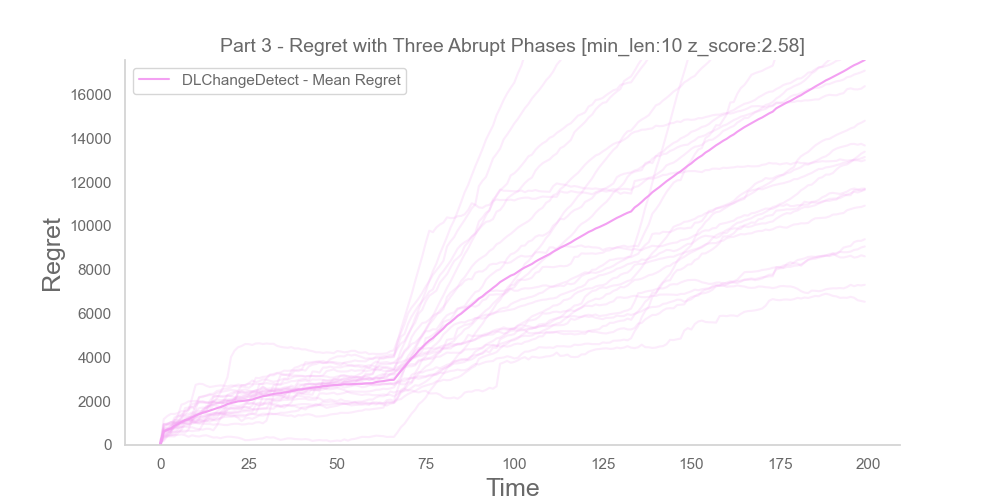
\includegraphics[width=\linewidth]{images/part3_min-len10_z_score2_58.png}
    \caption{case of min\_len = 10}\label{minlen10}
    \endminipage\hfill

    \caption{Selection of the best min\_len hyperparameter.}
    \label{minLenValidationFig}
\end{figure}



Differently from before, in this case the performance is not affected from the choice of the min\_len parameter and for this reason, in the final study, we have chosen to run the algorithm by setting min\_len equal to 10, because in this way we consider the arms with more data and so the test can be considered more reliable


\section{Performance evaluation}

This section aims to compare and describe the performance of the three described algorithms.
It is important to remark that in light of the validation we have performed, the comparison are between the standard version of the GP Learner, the Dynamic Learner implementing the sliding window mechanism with window length equal to 33, i.e. on third of the total time horizon of 200 days and the DL Change Detect learner with min\_len set to 10.
In particular three scenario have been tested:

\begin{enumerate}
    \item Three abrupt phases, each phase with a different length.
    \item Three abrupt phases, all the phases having the same length.
    \item Four abrupt phases with different length.
\end{enumerate}

The first scenario is intended to analyze and compare the performance of the three different algorithms, while the last two are more specific use cases aimed to compare the behaviour of the Dynamic Learner and the DL Change Detect learner and to show that the considerations made before actually occur.\\
In Figure \ref{regretPart3CompleteFig} the result of the first scenario is shown. As we can notice, except for the first days in which we have the first phase and so all the learner works similarly, the standard version of the GP Learner tends to increase linearly as the number of days increases. On the other hand the two dynamic algorithms both adapts very well to the abrupt changes of the non stationary environment and tend to grows logarithmically. In the plot, we can also see that in this case the DL Change Detector quickly fits the changes while the sliding windows mechanism is slower to learn the changes. Moreover we have that the second phase was very short and this affected drastically the performance of the Dynamic Learner and this is consistent to what seen before, because the behaviour of the algorithm depends on the length of the window.

\begin{figure}[!htb]
    \centering
    %\captionsetup{justification=centering,margin=1cm}
    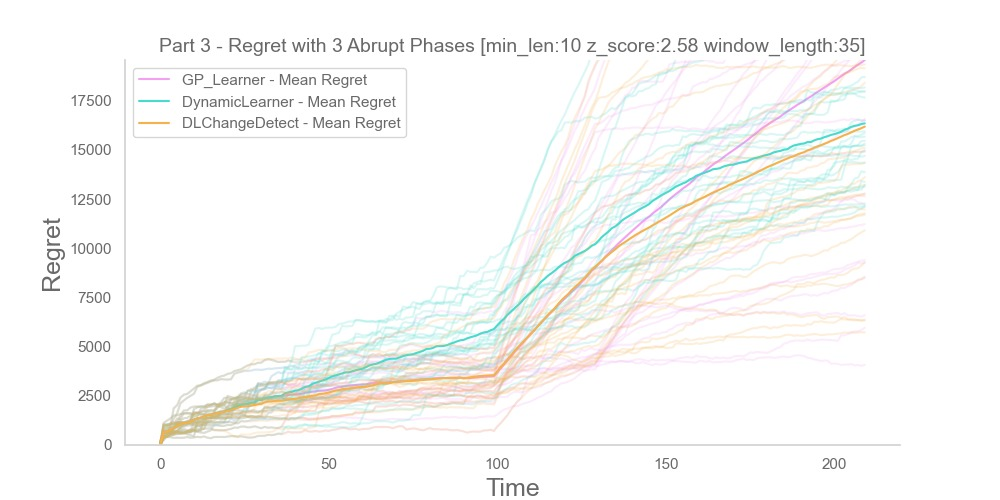
\includegraphics[width=\textwidth]{images/CompleteThreeDifferentPhases.jpeg}
    \caption{Comparison of the three implemented algorithms in non stationary environment}.
    \label{regretPart3CompleteFig}
\end{figure}

Finally, as already mentioned, two more specific use cases have been considered. In the following figures we can see the comparison of the regrets of the two implemented algorithms. More precisely in figure \ref{comparisonPlot1} the case of three phases, in which each phases consists of 66 days for a total time horizon of 200 days, while in figure \ref{comparisonPlot2} the scenario of four different phases more precisely of 50, 20, 90 and 40 days.\\ As we can see from the two plots, the DL Change Detector always outperforms the Dynamic Learner.

\begin{figure}[!htb]
    \centering
    %\captionsetup{justification=centering,margin=1cm}

    \begin{subfigure}[!H]{0.8\textwidth}
        \centering
        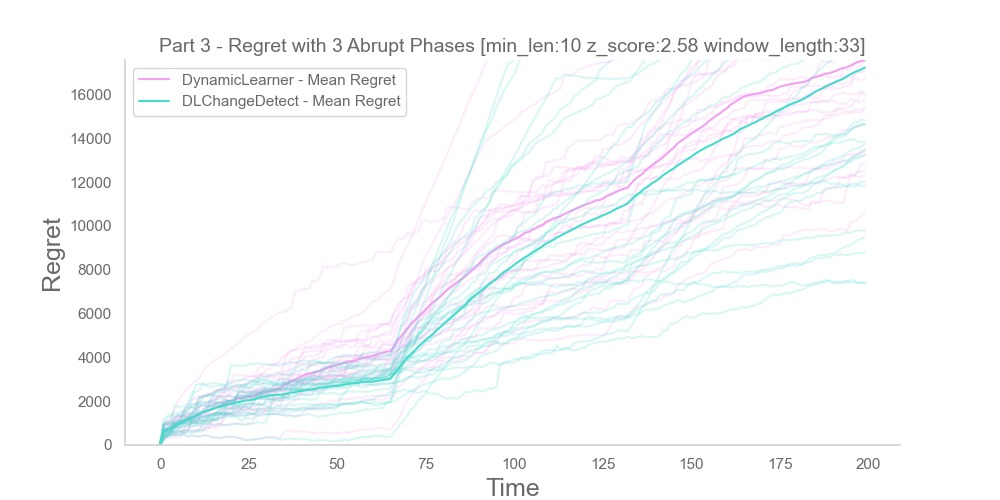
\includegraphics[width=\textwidth]{images/ThreeSamePhase.jpeg}
        \caption{Performance in scenario with three phases with same length}
        \label{comparisonPlot1}
    \end{subfigure}
    %\hfill
    \begin{subfigure}[!H]{0.8\textwidth}
        \centering
        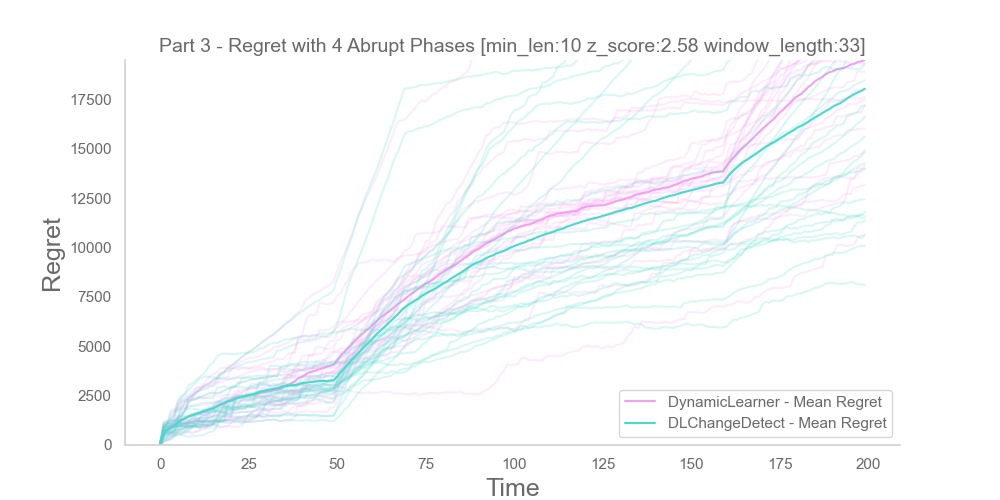
\includegraphics[width=\textwidth]{images/FourAbrupt.jpeg}
        \caption{Performance in scenario with four different phases}
        \label{comparisonPlot2}
    \end{subfigure}

    \caption{Comparison between the regrets of the Combinatorial bandit algorithm with a sliding window mechanism and of the Change Detector}
\end{figure}

    \newpage
    \chapter{Pricing: Learning the Best Price}

In this chapter we are going to focus our attention on the pricing and on the optimal price, that we can propose to our customers, to maximize the total revenue.

In common scenarios, in which there is a seller that has to sell products, the retail price is fixed without exploiting information from the buyers.
Sometimes, in physical markets, the customers have the possibility to negotiate and a skillful seller can maximize his revenue keeping the price as high as possible. This is a common practice, but experience is needed, to understand the limit of the buyers, and moreover it requires time, loosing the possibility to serve other clients.

In e-commerce scenarios, we can do better exploiting information from the users, from the big data and from the software automation.
In particular, given the assignments~\ref{assPart4}, we are going to design an algorithm being able to learn the optimal price for our product, to maximize the total revenue.

In the following steps, we are going to:
\begin{itemize}
    \item define the demand curves of the users.
    \item describe the environment setup.
    \item explain the algorithm that has been chosen.
    \item comment the results obtained in the end of the campaign.
\end{itemize}


\section{Demand Curves}

In the economic literature is defined the concept of \textbf{demand curve}.
It is a function that maps the price to a certain probability. In other words, given a price, the function returns the probability that the product will be sold. Therefore, if we plot the demand curve, we'll obtain on the x-axis the admissible prices and on the y-axis the probability (between $0$ and $1$).

In our simulated scenario, we defined three classes of users with the corresponding demand curves. The shapes of the curves are motivated by the intrinsic behaviors of the classes:
\begin{itemize}
    \item \textit{Elegant}: they are rich, they are looking for luxury products, thus they find no interest in products with low prices. Their interest grows as the price rises, but the odds of buying remain low.
    \item \textit{Casual}: they are students, thus they are able to buy the product only if the price is relatively low.
    \item \textit{Sports}: they are workers, but without a particular interest on the shoes, therefore the price is relatively irrelevant and the probability is low. Only if the price becomes really high, they completely lose interest.
\end{itemize}

In figure \ref{demandCurvesFig} there are the curves designed following the above descriptions.
\footnote{A tool as been implemented to draw the curves manually. It requires few points and it performs polynomial regression to augment the sampling definition. It can be found in the attached code.}

In the same figure, the \textit{aggregate} curve has been reported (colored in \textit{orange}), it represents the mean between the other curves. (It will be useful in the next subsections.)
Moreover, points representing the theoretical optimum are reported. The area below them is maximum w.r.t. the curves.

\begin{figure}[H]
    \centering
    %\captionsetup{justification=centering,margin=1cm}

    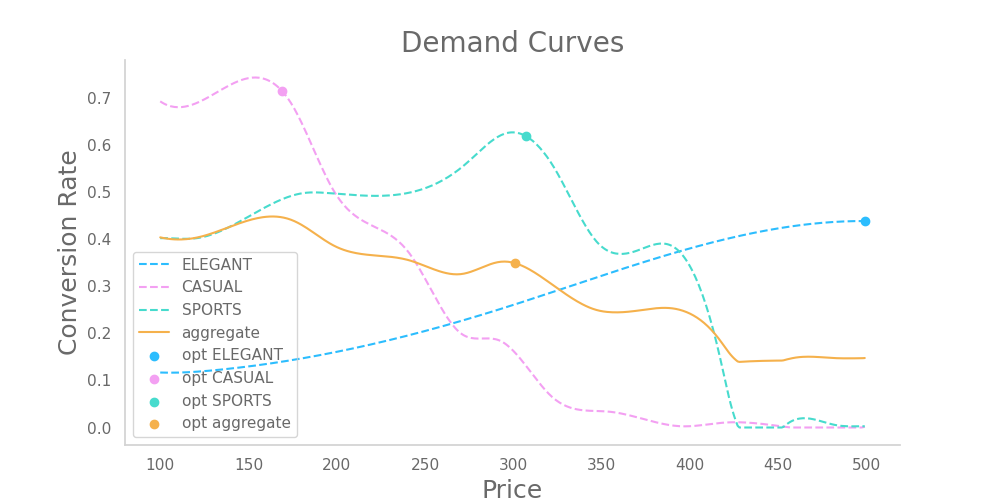
\includegraphics[width=1.0\textwidth]{images/demand_curves.png}
    \caption{\textbf{Demand Curves}.\\
    They are used to model the probability (\textit{conversion rate}) that a certain class, of customers, will buy or not the product w.r.t. a proposed price.\\
    The dashed lines represent the demand curves of the corresponding classes:
    \textit{blue} for the \textit{Elegant} class.
    \textit{pink} for the \textit{Casual} class.
    \textit{light green} for the \textit{Sports} class.\\
    The \textit{orange} curve is the mean between the others and it is used to study the \textit{aggregate} model.\\
    The points are displayed to show the optimal price w.r.t. the conversion rate: the area below them is maximum.}
    \label{demandCurvesFig}
\end{figure}


\section{Environment}

In our implementation, the environment is a black box from the point of view of the learning algorithm.
It is used to iterate over the days, for the entire duration of the campaign.
It schedules the time and the number of users reaching our theoretic website.

Every user is randomly taken from the three classes and the class is not communicated to the learner. The environment, knowing the original class of the users, computes the optimal revenue and returns the effective reward obtained by the learner.
How the learner will handle these information will be explained in the next subsections.


\section{Learner Algorithm Selection}

This context of application can be solved in different ways, but the most common choice is to use a \textit{multi-armed bandit (MAB)} algorithm.

We mainly tested two algorithms:
\begin{itemize}
    \item \textbf{Thompson Sampling (TS)} algorithm.
    \item \textbf{Thompson Sampling with Sliding Window (SWTS)} algorithm.
\end{itemize}

We tested both the algorithms during the implementation phase, but since the SWTS is more sensible to the window size, and finding a good one requires a lot of testing, we kept the TS as final choice.\\
This decision has been motivated by the fact that there aren't abrupt phases, thus there is no impelling reason to "forget the past" as done by SWTS.

An additional note must be done for the pulling phase of the TS algorithm. The standard implementation of the TS pulls the arm in this way:
\begin{equation}
    a_t \leftarrow \argmax_{a \in A} \{\tilde{\theta}_a\}
\end{equation}
Where $A$ is the set of arms; $\tilde{\theta}_a$  is the sampled random value from the beta distribution for arm $a$.\\
This implementation maximize the demand, but since we are interested in the maximization of the total revenue, we pull the arms as below:
\begin{equation}
    a_t \leftarrow \argmax_{a \in A} \{\tilde{\theta}_a \cdot price_a\}
\end{equation}
Where $price_a$ is the price targeted by the arm $a$.\\
This allow us to maximize the area under the demand curve.


\section{Performance Evaluation}

Summarizing, we have to learn the best price to propose, to the users, to maximize the total revenue.\\
We have discussed about the environment, that generates incoming users and allows us to iterate over the days of the campaign, and finally, we presented the learner adopted.
At this point we can explain how the tests have been initialized.

The experiments has been configured in two ways:
\begin{itemize}
    \item keeping a fixed daily price: we pulled an arm only for the first user of the day, for the other users we proposed always the same price. This means that for the entire day we pull and update always the same arm of the TS.
    \item one price for each user: maybe, this is an unpractical option in a real world scenario, but it allows to obtain a total revenue outperforming the previous configuration. This method achieves better performances since the learner is updated more frequently during the campaign.
\end{itemize}

In the end of the tests, the figure \ref{regret4Fig} reports the obtained regrets. The sub figure \textit{(a)} for the first configuration and the sub figure \textit{(b)} for the second.

We plotted two regrets computed with two different optimal revenues.
The regret called \textbf{Mean Regret of the Aggregate Model} has been computed using, as optimal, the optimal point taken from the aggregate model. This is an optimistic regret because it doesn't take into consideration the information about the specific class of the users. In other words, the learner and the clairvoyant algorithm don't know the class of the customers.

The learner is learning the aggregate model, thus this comparison seams fair, but since the clairvoyant knows the original class of the users, we introduced the so called \textbf{Mean Regret of the True Evaluation}. Obviously, from the point of view of the learner, this is a pessimistic computation since it is unable to infer more information from the input data.

Anyway, these two ways to compute the regrets will be useful in the next chapter, since the learner will be able to infer more information from the data creating contexts to exploit a finer profiling.
You will notice how the two regrets will be pushed down and the regret on the True Evaluation will be more similar to the regret of the Aggregate Model obtained here, proving that a finer profiling improves drastically the performances.


\begin{figure}[!htb]
    \centering
    %\captionsetup{justification=centering,margin=1cm}

    \begin{subfigure}[!H]{0.8\textwidth}
        \centering
        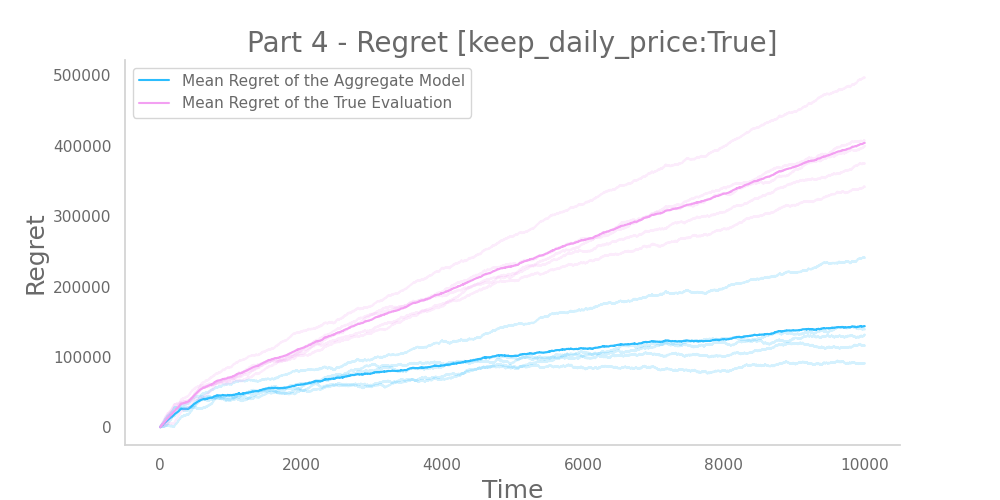
\includegraphics[width=\textwidth]{images/part4_keep-daily-priceTrue.png}
        \caption{Regret obtained proposing to the customers the same price for the entire day.}
    \end{subfigure}
    %\hfill
    \begin{subfigure}[!H]{0.8\textwidth}
        \centering
        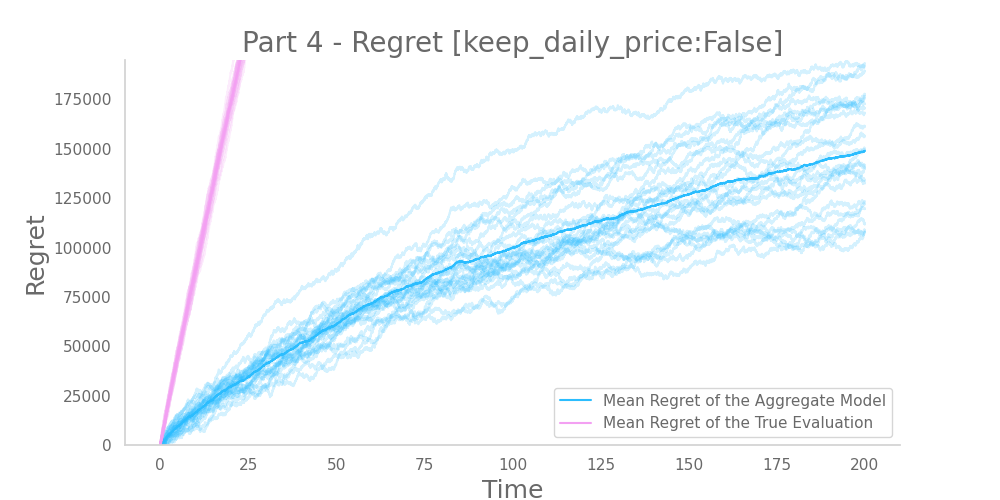
\includegraphics[width=\textwidth]{images/part4_keep-daily-priceFalse.png}
        \caption{Regret obtained proposing to the customers different prices for each visit.}
    \end{subfigure}

    \caption{Comparison between the regrets obtained during the campaign.\\
    The \textbf{Mean Regret of the Aggregate Model} (colored in \textit{blue}) is the regret computed keeping, as optimal, the area under the optimal point of the aggregate curve~\ref{demandCurvesFig}. In other words, both the learner and the clairvoyant don't know the class of the customers. This is an optimistic measure of the regret.\\
    The \textbf{Mean Regret of the True Evaluation} (colored in \textit{pink}) is the regret obtained computing the optimal value exploiting the original class of the customers.}
    \label{regret4Fig}
\end{figure}
    \newpage
    \chapter{Pricing: Context Generation}\label{ch:pricing:-context-generation}

In this chapter we want to further expand what we have seen in the previous one.
In the general case, since we have access to many information about our clients, we can not only identify different classes of users, with different buying powers, but also understand to which class a new user belongs, based on the information we have about him (given, for example, by cookies).
The idea is to exploit this knowledge in order to charge different prices to each class and so maximize our revenue.
To do so, we will use the idea of the \textbf{context}, which will be explained in the next section.
We will then explain the differences in the environment used in this chapter, tackle the approaches we followed to create the algorithm and analyze the final results.


\section{What is a Context?}\label{sec:what-is-a-context?}
As said before, in this scenarios we have a lot of information about the users that visit our website, so we can group them together in classes.
Usually a class is identified by a single value (or subsets of values) for each feature.
The issue is that the number of classes grows exponentially with the number of features, making unfeasible the problem of defining and optimizing a single price for each class when we have many features for each user (which is the most common scenario in real cases).
A context is a partition of the feature space according to some values of the features (for example a male with age between 18 and 24 is a context), grouping together various classes.
By using contexts instead of classes, we are able to drastically reduce the number prices we have to decide, so the problem can be tackled and solved in a reasonable time.


\section{Environment, Learner and Demand Curves}\label{sec:environment,-learner-and-demand-curves}
The environment is fairly similar to the one used in Chapter 4, the only difference is that it keeps track of how many days have passed since the collected data has been analyzed, so that we know when we have enough to consider generating the new contexts.
This is possible because we know how many users will visit our website every day, so we know exactly how much data we have after each day.
We used the same demand curves as in Chapter 4, on the other hand, since we want to learn different prices now, we don't use a single learner anymore, but we create a new SWTS one with each new context.


\section{Campaign Scheduler}\label{sec:campaign-scheduler}
The class Campaign Scheduler acts as the main interface for our algorithm.
It stores the contexts we are currently using for the week and the information collected by our website so far in the following structure, indexed using the classes we have chosen.
\begin{itemize}
    \item \textit{Total Reward}: The sum of all the rewards we have obtained so far.
    \item \textit{Number of purchases}: The number of products we have actually sold.
    \item \textit{Number of users}: The number of users who have visited our website.
    \item \textit{Rewards}: An array that contains all the rewards collected so far.
\end{itemize}
These information are updated after each user visits the website and will then be used in the Context Generator class to decide whether to create new contexts or not.


\section{Our Approach to Context generation}\label{sec:our-approach-to-context-generation}
When we first approached the problem, we used a algorithm with a greedy approach.
We start with the aggregate model, so we have only one price for all the classes, and we use it to collect data for the first week.
At the end of the week, we use this data to evaluate the features and decide if we want to split and generate new contexts.
For each feature that we have yet to use to split, we compute the lower bound of the probability of the context to occur and of the expected reward.
This is because when we create a new context, we have to learn a different model, which will surely have more uncertainty with respect to the one used so far.
The lower bound is a measure of how much we are guaranteed to gain, the reward we collect in the end might be higher.

For the lower bound of the probability we used the Hoeffding bound since the probability has limited values.

\begin{equation}
    x - \sqrt{-\frac{\log_n{d}} {2 n}}
\end{equation}
where:
\begin{itemize}
    \item $n$ : is the number of samples.
    \item $x$ : is the mean of the rewards.
    \item $d$ : is a value that defines how much confidence we want.
\end{itemize}

For the reward we had to use a different formula, since its values are unlimited.

\begin{equation}
    x - t \sqrt{\frac{sq} {n}}
\end{equation}
where:
\begin{itemize}
    \item $n$ : is the number of samples.
    \item $x$ and $sq$ : are the mean and variance of the real rewards.
    \item $t$ : is a value that defines how much confidence we want.
\end{itemize}

After evaluating the expected reward relative to each feature, we select the one with the highest value and compare it with the expected reward of the current model.
If it is larger or equal we create the new contexts, if not we keep the previous model and start a new week.
This process is iterated week after week, without a termination condition, because we are continuously collecting information which might change how our contexts are organized.
In the general case this algorithm does not guarantee optimality and is used to solve scenarios in which we have many features with possibly many values thanks to its performances.
On the other hand it gives us some insight on which features might be the most important in the scenario.

However our problem was quite different from the general one, so we chose a different approach: evaluating every week the entire set of possible partitions.
Since we have only two features with binary values, this process is not computationally heavy and we can use this solution with reasonable time performances.
We always start with the aggregate model to collect data, but when the time to split arrives, we evaluate all possible partitions of our feature space, using the above formulas.
This way we can either obtain the aggregate model, two or three contexts, by not splitting, splitting according to only one or both features (we would obtain four contexts, but we only have three classes).


\section{Performance Evaluation}\label{sec:performance-evaluation-5}

As in Chapter 4, we configured the experiment to both keep the same price for the day and not to and this is the reason of the two graphs.
Moreover we used the same two optimal models, the Aggregate Model, which does not know the classes of the users, and the True Evaluation, which does and chooses a single price for each of them.
This was done to compare the results of the algorithms we have built.

As we can see in figure \ref{regret5Fig}, the algorithm largely outperforms the Aggregate Model, because it knows the classes of the users and can choose a price for each of them.
In the first weeks we observe a small growth before the decrease, this is because the algorithm starts from the aggregate model and is still learning the correct prices.
We can also see that the initial growth lasts longer when we keep a daily price, because by fixing the price it takes longer to learn the curve.
This comparison was mainly done to show the improvements with respect to the algorithm in Chapter 4.
On the other hand, the True Evaluation model performs better than the algorithm in the first weeks, but as time goes on the difference becomes smaller and smaller, as the algorithm learns the best prices.

\begin{figure}[!htb]
    \centering

    \begin{subfigure}[!H]{0.8\textwidth}
        \centering
        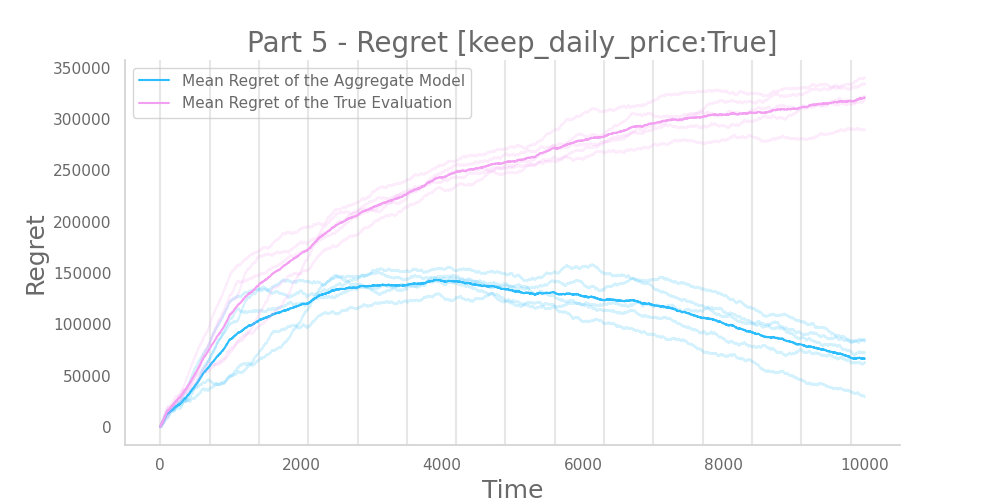
\includegraphics[width=\textwidth]{images/part5_keep-daily-priceTrue.png}
        \caption{Regret obtained proposing to the customers the same price for the entire day.}
    \end{subfigure}

    \begin{subfigure}[!H]{0.8\textwidth}
        \centering
        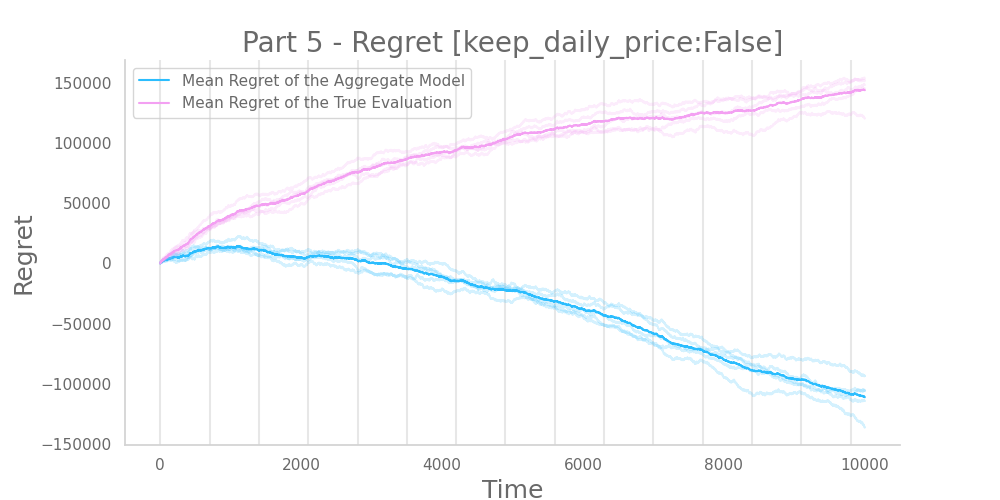
\includegraphics[width=\textwidth]{images/part5_keep-daily-priceFalse.png}
        \caption{Regret obtained proposing to the customers different prices for each visit.}
    \end{subfigure}

    \caption{Comparison between the regrets obtained during the campaign.\\
    The \textbf{Mean Regret of the Aggregate Model} (colored in \textit{blue}) is the regret computed keeping, as optimal, the area under the optimal point of the aggregate curve~\ref{demandCurvesFig}.\\
    The \textbf{Mean Regret of the True Evaluation} (colored in \textit{pink}) is the regret obtained computing the optimal value exploiting the original class of the customers.\\
    The vertical lines are positioned every seven days, to underline when the new weekly contexts are generated.}
    \label{regret5Fig}
\end{figure}

    \newpage
    \chapter{Adverting and Pricing Integration}

Reached this point the goal is to attract the most valuable users, that is allocate the budget during Advertising so that it is focused on attracting users that will maximize the total reward; this expectation on the reward is modeled by the pricing algorithms presented before. In this section we will present how we have modeled the intregation between Pricing and Advertising section, which are the algorithm proposed and an analysis of the final results.

\section{Proposed Integration}
The idea behind our integration is to have, for each Subcampaign, the possibility to manage separately the Advertising and the Pricing in order to reuse all the algorithms presented in the previous sections and, on top of it, build a Budget Allocator that is able to collect all the information and calculate the best allocation of the budget. The complete flow chart can be found at \ref{fig:part6scheme}, in the following we will discuss it step by step.

    \subsection{Budget Allocator}
    Every day, this component is the one that, collected information from the past, calculates the best budget allocation. Initially, when we have no historical information, it is built to output a balanced allocation among all the Subcampaigns. After the initialization phase, evey new day, it collects for every subcampaign $ j $ two values:
    
    \begin{enumerate}
        \item $ n_j (.) $ : Learned distribution of clicks over budget allocation for subcampaign $ j $. This function comes from the regression generated by the GPTS learner in the   \textbf{Advertising} section.
        \item $ v_j $ : Learned value, in terms of expected reward for subcampaign $ j $. This value comes from the evaluation of the collected reward during the last days in the \textbf{Pricing} section.
    \end{enumerate} 

    At this point we are able to define the Knapsack Optimization Problem as: 

    \begin{equ}[!ht]
        \begin{equation*}
            \max_{y_j,_t} \sum_{j=1}^{N} v_j n_j(y_j,_t)
        \end{equation*}
        \begin{equation*}
            \sum_{j=1}^{N} y_j,_t \leq \bar{y}_t
        \end{equation*}
        \captionsetup{labelformat=empty}
        \caption{The complete legend can be found at Figure \ref{fig:part6scheme}}
    \end{equ}


    \subsection{Advertising}
    For each subcampaign $ j $, given the budget allocation $ y_j,_t $, it is possible to collect from the environment the real number of clicks $ N_j(y_j,_t) $ generated by this allocation and update, as we have done in Chapter 2 and 3, the GPTS learner.
    At the end it is returned the distribution $ n_j(.) $ learned by the Gaussian Process.

    
    \begin{figure}[H]
        \centering
        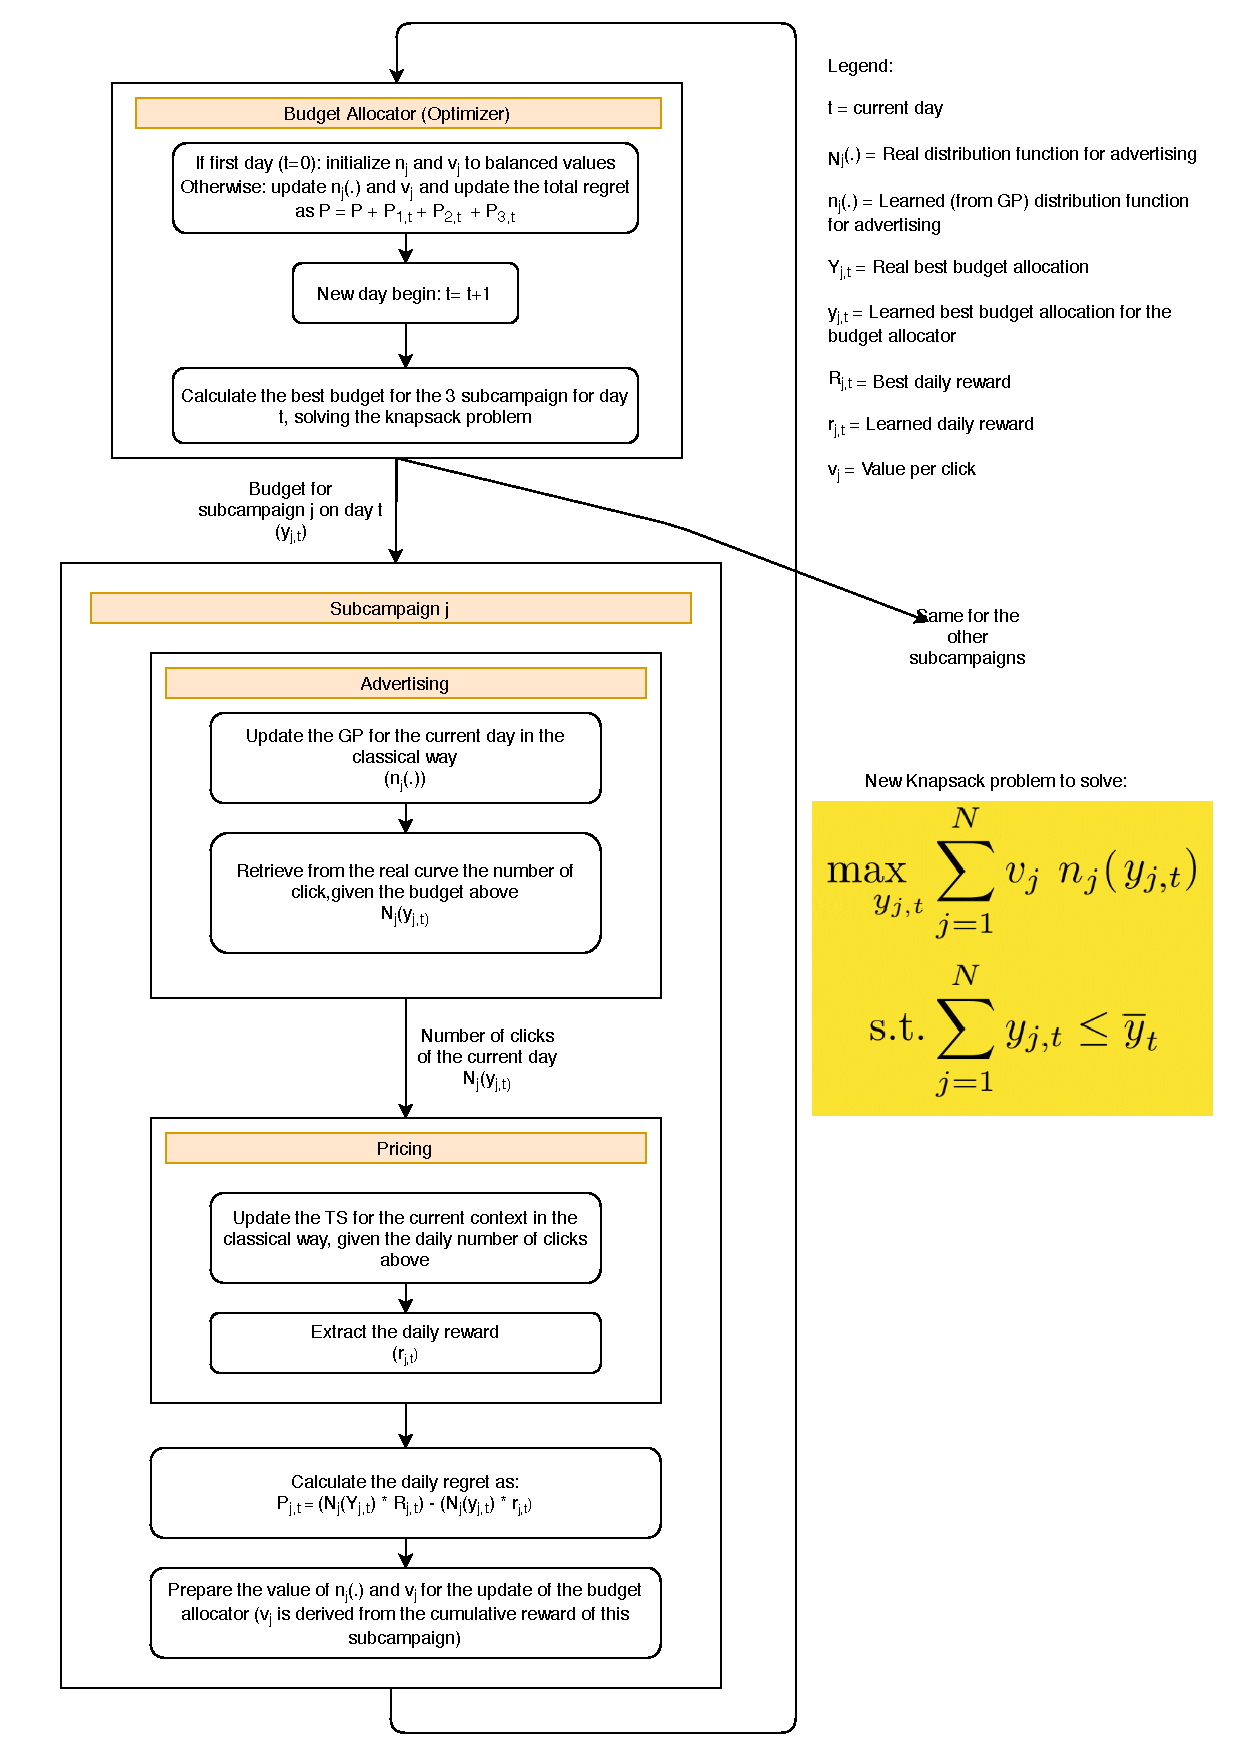
\includegraphics[scale=0.8]{images/part6_schema.pdf}
        \caption{Flow Chart Diagram of part 6}
        \label{fig:part6scheme}
    \end{figure}


    \subsection{Pricing}
    For each subcampaign $ j $, given the real number of clicks $ N_j(y_j,_t) $ generated by the \textbf{Advertising}, it is possible to collect the real revenue $ r_j,_t $ fot the current day and update, as we have done in Chapter 4, the TS learner.
    \newpage
    \chapter{Advertising and Pricing: Fixed Prices}

The goal of this final part is the maximization of the total reward by attracting the most valuable users through the Advertising algorithms in a scenario where it is not possible to choose a different price for each class of user. In this scenario, differently from what we have seen in chapter 6, we have a further constraint that the seller charges a unique price to all the classes of users and so we cannot find what is the best price for each subcampaign as we did before, but we have to find a \underline{unique} optimal price able to maximize the revenue for all the subcampaigns.\\ In the following sections we go through the reward maximisation algorithms we implemented to choose the best price for all the users that together with the Adverting will bring the best possible reward.


\section{Proposed Integration}
The main idea to solve the described problem is to iterate over all the possible prices in order to choose the one that jointly with the corresponding advertising optimization will produce the best reward.
To achieve this goal we updated the \textbf{\textit{Budget Allocator}} implemented in part 6 which in this new scenario iterates over all the possible prices and thanks to the information received by the \textbf{\textit{Sub Campaign Handlers}} \footnote{The Sub Campaign Handler is a component in charge to learn both the advertising curve and the demand curve associated to a specific sub campaign} it computes the best budget allocation which will be used jointly to the price to estimate the corresponding number of purchases and relative revenue. At the end of this iteration the Budget Allocator will choose the optimal price, that is the one with the greatest estimated reward and it will propose it to the users the next day combined with the already computed allocation for the advertising sub campaigns.\\ This problem has been tackled with two different approaches, the first one based on a \textit{Bernoulli} model, while the second one based on a \textit{Normal} model. Both implemenations will be better described in the following sections. \\It is important to remark that also in this scenario the main idea was to decompose, wherever feasible, the two problems, namely the Advertising and Pricing, in order to reuse as much as possible all the algorithms presented in the previous chapters.

\section{First implementation: based on Bernoulli distribution}
In our first implementation we approached the Pricing problem exploiting the algorithm already implemented for the previous problems. More precisely in this implementation every time a new user enters on the website, the Environment determines if she will buy or not the item, by making an extraction from a \textit{Bernoulli distribution}. Under this assumption we could reuse the \textit{Thompson Sampling} algorithm already implemented for solving the pricing problem on Part 4.
While for learning the Advertising curves associated to each subcampaign we used the GPTS already implemented for solving the Advertising subproblem as we did in part 6.\\ The performance of the implemented algorithm is for now postponed and it will be analyzed in the last section, after the description of the second approach we went through.


\section{Second implementation: based on Normal distribution}
For the second implementation we started from the consideration that under certain constraintrsints the binomial distribution is well approximated by the normal distribution. Let's consider the binomial distribution defined by the function:
\begin{equation}
    f(x) = \frac{n!}{x!(n-x)!}  p^x q^{n-x} 
\end{equation}

which represents the probability of exactly x successes in n indipendendet Bernoulli trials where a given trial has two possible outcomes, that is a "success" and a "failure"\footnote{In our scenario a success is when the user purchases the item once he visits the website, while a failure if she doesn't} respectively with probability \textit{p} and $q=(1-p)$.\\ When \textit{n}, \textit{np} and \textit{nq} are large, then the binomial distribution is well approximated by the normal distribution:
\begin{equation}
    f(x)  \sim \frac{1}{\sqrt{2 \pi npq}} e^{ \frac{-(x-np)^2}{2npq} }
\end{equation}

Since we are working with very large value of n, we can procede with such approximation without worrying about the value of \textit{np} and \textit{nq}.
So we can consider the case in which the pricing Environment is based on a \textit{Normal distribution}. Under these considerations, all the information are collected at the end of the day and no more at each visit. In this way the number of purchases will be considered as an aggregation of Bernoulli extractions.
In this second implementation the curves associated to the Pricing and Advertising subproblems are both learned by using the GPTS algorithm already implemented.\\
Differently from the previous implementation in which we collected the information after each visit of a user, in this case we learn the approximated distribution and so we could have more problems with suboptima. To solve this problem we have introduced the concept of \textbf{\textit{artficial}} \textbf{\textit{faiding}}\footnote{The noise decreases as the number of days increases} \textbf{\textit{noise}}, i.e. a random noise added to the confidence of the arms once they are pulled. Indeed using the Gaussian Process to learn the curves we have more problems to find the best solution to the Exploration$\backslash$Eploitation trade-off dilemma because we have more possibilities to discard the true optimal arm. By adding this fictitious noises we will increase the exploration phase and in this way we avoid that the algorithm focuses on a suboptimum.\\ It is important to remark that,since we use the GPTS algorithm to solve both the Pricing and Advertising subproblems, the noise has to be added to both the curves learned by the corresponding learners.\\ During the perfomance evaluation in the next section we will compare the behaviour of this implementation with respect to the first one and we will analyze the difference we have by running this algorithm with and without the artificial noises.

\section{Performance Evaluation}
This section aims to compare and describe the performances of the above described algorithms. In Fig. \ref{regretPart7Binomial} we can see the regret associated to the first described algorithm, that is in the case in which the Environment make an exactraction from a Bernoulli distribution every time a new user visits the page. 

\begin{figure}
    %\captionsetup{justification=centering,margin=1cm}
    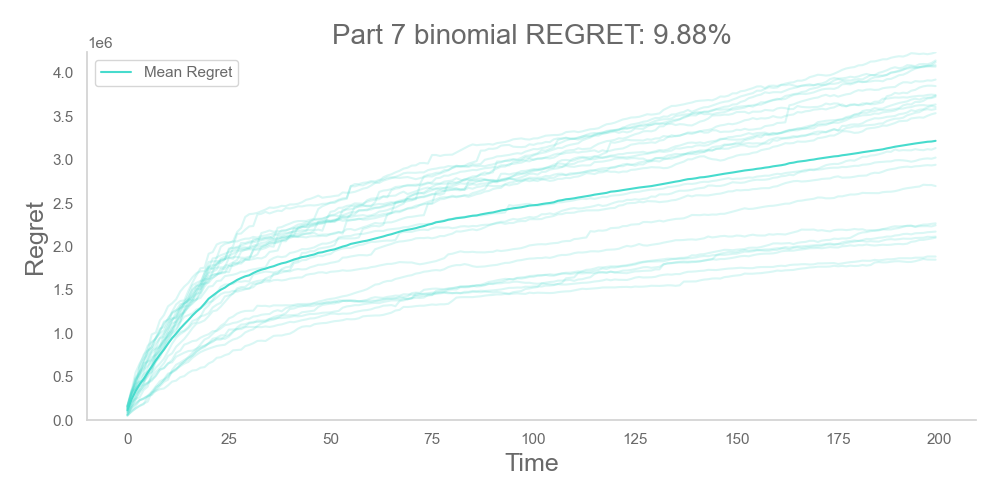
\includegraphics[width=\textwidth]{images/part7_binomial_regret.png}
    \caption{Regret obtained when we consider an Environment which makes Bernoulli extractions}
    \label{regretPart7Binomial}
\end{figure}

In Figure \ref{fig:RegretsPart7Normal} we show the regret associated to the second implementation, that is in the case in which the Environment collects the information from an approximated Normal distriution. In the figure we can also see how, in this scenario, the performance changes varying the value of the artificial noises.

\begin{figure}[!htb]
    \centering

    \begin{subfigure}[!H]{0.8\textwidth}
        \centering
        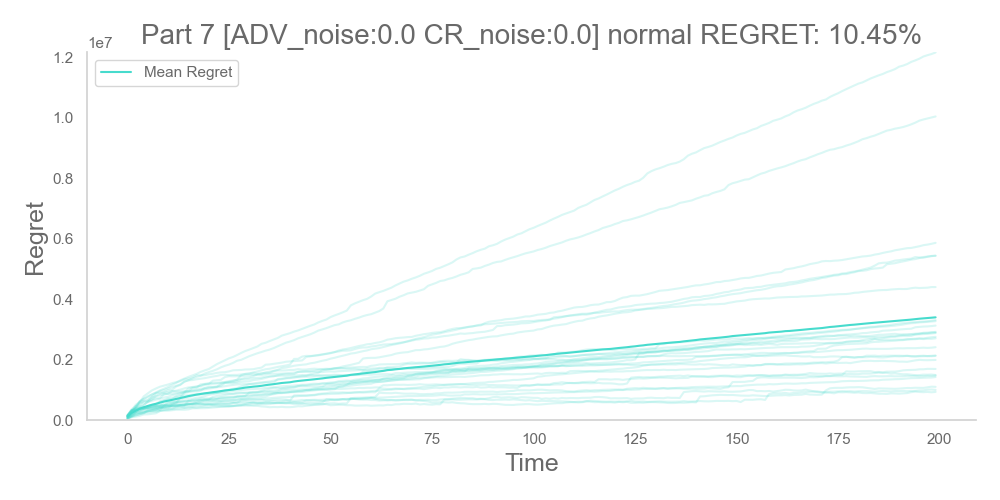
\includegraphics[width=\textwidth]{images/part7_normal_regret_noise00.png}
    	\caption{Regret without artificial noise}
    \end{subfigure}

    \begin{subfigure}[!H]{0.8\textwidth}
        \centering
        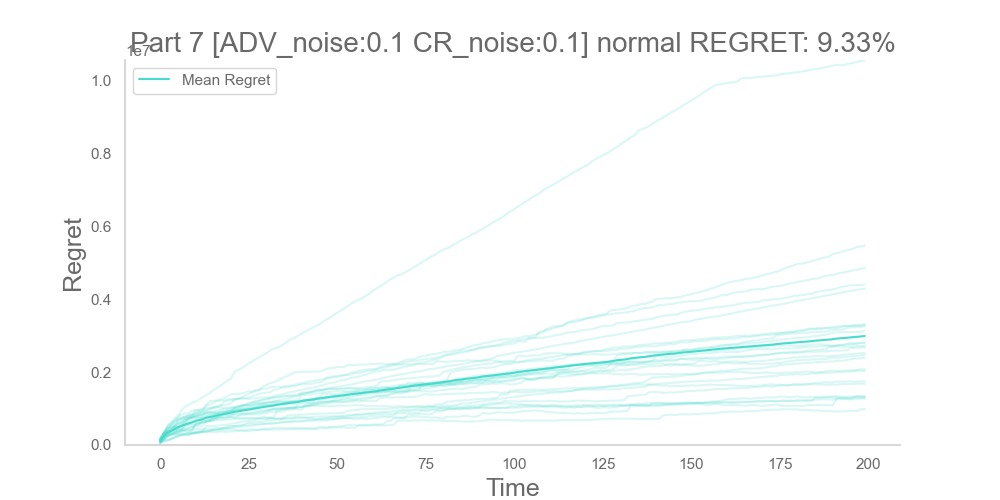
\includegraphics[width=\textwidth]{images/part7_normal_regret_noise01.jpeg}
    	\caption{Regret with artificial noise equal to 0.1}
    \end{subfigure}
    
    \begin{subfigure}[!H]{0.8\textwidth}
        \centering
        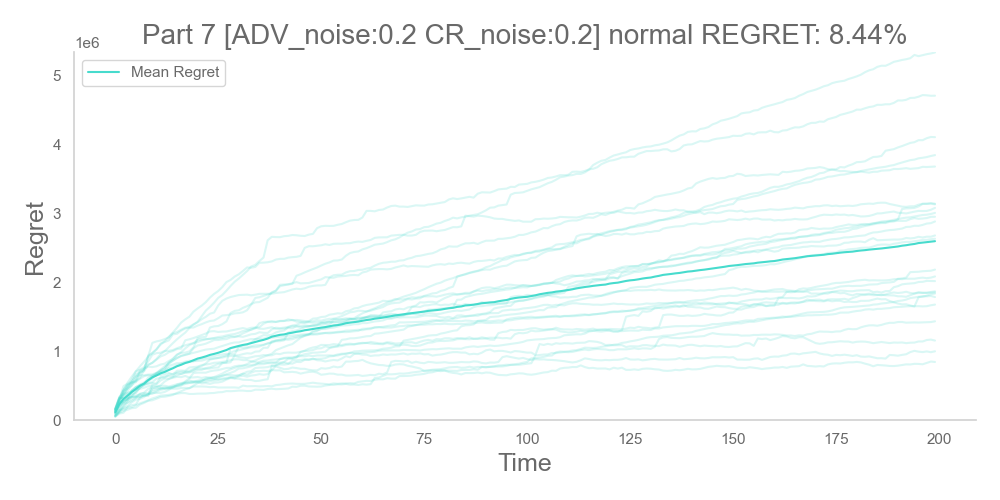
\includegraphics[width=\textwidth]{images/part7_normal_regret_noise02.png}
    	\caption{Regret with artificial noise equal to 0.2}
    \end{subfigure}
    
    \caption{Comparison between the regrets with and without the artificial noises when we consider an Environment based on a Normal distribution}
    \label{fig:RegretsPart7Normal}
\end{figure}
    \newpage
    \chapter{Assignments}

Part 2:
\textit{Design a combinatorial bandit algorithm to optimize the budget allocation over the three subcampaigns to maximize the total number of clicks when, for simplicity, there is only one phase. Plot the cumulative regret.}
\label{assPart2}\\

Part 2:
\textit{Design a sliding-window combinatorial bandit algorithm for the case, instead, in which there are the three phases aforementioned. Plot the cumulative regret and compare it with the cumulative regret that a non-sliding-window algorithm would obtain.}
\label{assPart3}\\

Part 4:
\textit{Design a learning algorithm for pricing when the users that will buy the product are those that have clicked on the ads. Assume that the allocation of the budget over the three sub campaigns is fixed and there is only one phase (make this assumption also in the next steps). Plot the cumulative regret.}\label{assPart4}

%\bibliographystyle{unsrt}  
%\bibliography{references}  %%% Remove comment to use the external .bib file (using bibtex).
%%% and comment out the ``thebibliography'' section.


%%% Comment out this section when you \bibliography{references} is enabled.
% \begin{thebibliography}{1}

% \bibitem{kour2014real}
% George Kour and Raid Saabne.
% \newblock Real-time segmentation of on-line handwritten arabic script.
% \newblock In {\em Frontiers in Handwriting Recognition (ICFHR), 2014 14th
%   International Conference on}, pages 417--422. IEEE, 2014.

% \end{thebibliography}


\end{document}document}